\section{Euclidea tools}
\begin{table}[!htb]
\begin{center}
 \setlength{\tabcolsep}{4pt}
 \begin{tabular}{ p{2.4cm} | p{3.2cm} | p{6.7cm} } 
 Tool & Arguments & Description \\
 \hline
 \newline &  &  \\
 Point &
 (coordinates) &
 Create a point using the first applicable rule from the following:
\begin{enumerate}
  \item Create a point on the closest intersection of primitives if there are any.
  \item Create a point on the closest geometric primitive if there are any.
  \item Create a point at the exact coordinates given by the argument.
\end{enumerate} \\
 Line &
 (point*, point*) &
 Draw a line passing through the given points.
 \newline \\
 Circle &
 (point, point) &
 Draw a circle centered at the first point with a radius marked by the second point.
 \newline \\
 Perpendicular Bisector &
 (point*, point*) &
 Draw the perpendicular bisector of two given points.% & 1 & 3 \\
 \newline \\
 Angle Bisector &
 (point*, point, point*) &
 Draw the axis of an angle, where the second point marks the vertex and the first and the third points lie on its rays. 
 \newline \\
 Perpendicular &
 (line, point) &
 Draw a line perpendicular to the line passing through the point.
 \newline \\
 Parallel &
 (line, point) &
 Draw a line parallel to the line passing through the point.
 \newline \\
 Compass &
 (point*, point*, point) &
 Draw a circle with a center in the third point and a radius given by the distance between the first two points. \\
\end{tabular}
\caption{Tools available for construction steps in Euclidea.
The asterisk denotes interchangeable arguments.}
\label{tab:description_of_tools}
\end{center}

\end{table}
\newpage
\section{Additional qualitative examples}
\label{more_examples}
\subsection{Level \textit{Gamma-08}}
\begin{figure}[!htb]
     \centering
     \begin{subfigure}[t]{0.32\textwidth}
         \centering
         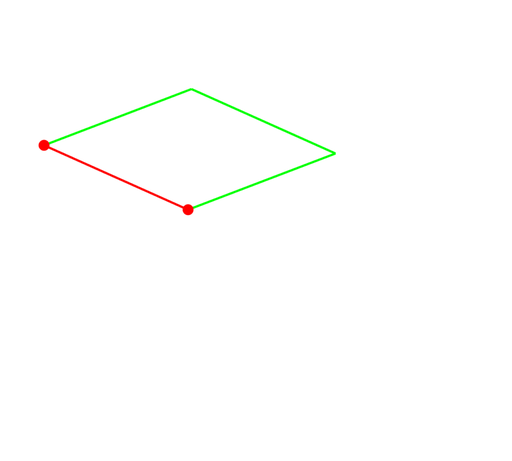
\includegraphics[width=\textwidth]{img/Gamma-08_example/input_image0.png}
         \caption{Input}
         \label{fig:Gamma08_example_input}
     \end{subfigure}
     \hfill
     \begin{subfigure}[t]{0.32\textwidth}
         \centering
         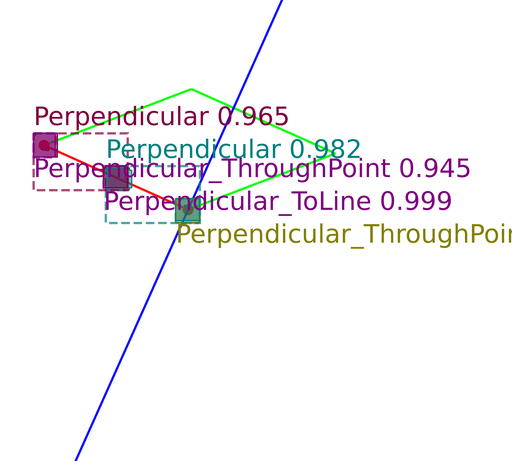
\includegraphics[width=\textwidth]{img/Gamma-08_example/output_image0.png}
         \caption{Step 1: Parallel tool}
         \label{fig:Gamma08_example_step1}
     \end{subfigure}
     \hfill
     \begin{subfigure}[t]{0.32\textwidth}
         \centering
         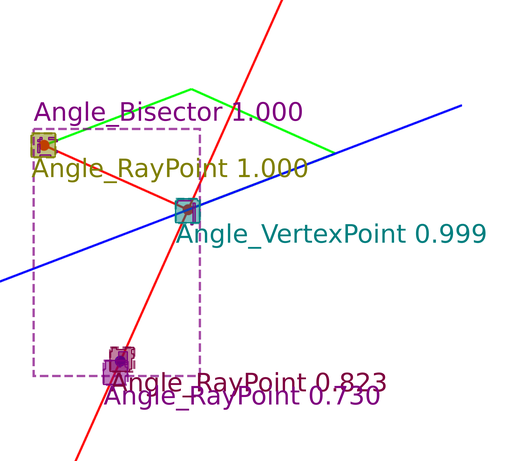
\includegraphics[width=\textwidth]{img/Gamma-08_example/output_image1.png}
         \caption{Step 2: Angle Bisector tool}
         \label{fig:Gamma08_example_step2}
     \end{subfigure}
     \hfill
     \begin{subfigure}[t]{0.32\textwidth}
         \centering
         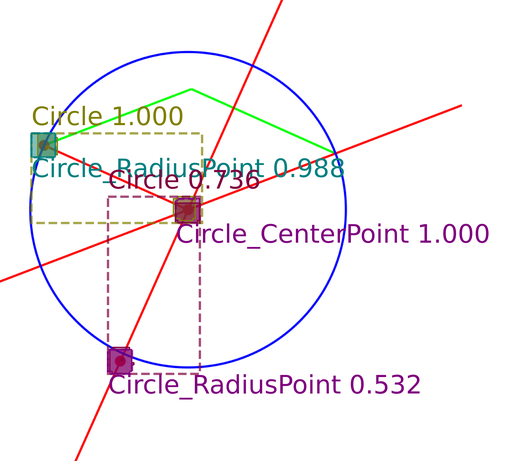
\includegraphics[width=\textwidth]{img/Gamma-08_example/output_image2.png}
         \caption{Step 3: Circle tool}
         \label{fig:Gamma08_example_step3}
     \end{subfigure}
     \hfill
     \begin{subfigure}[t]{0.32\textwidth}
         \centering
         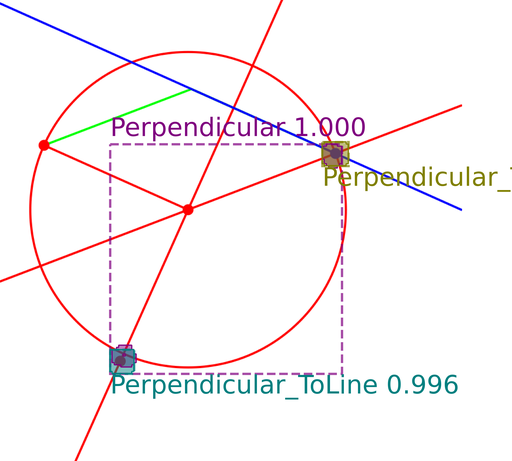
\includegraphics[width=\textwidth]{img/Gamma-08_example/output_image3.png}
         \caption{Step 4: Perpendicular tool}
         \label{fig:Gamma08_example_step4}
     \end{subfigure}
     \hfill
     \begin{subfigure}[t]{0.32\textwidth}
         \centering
         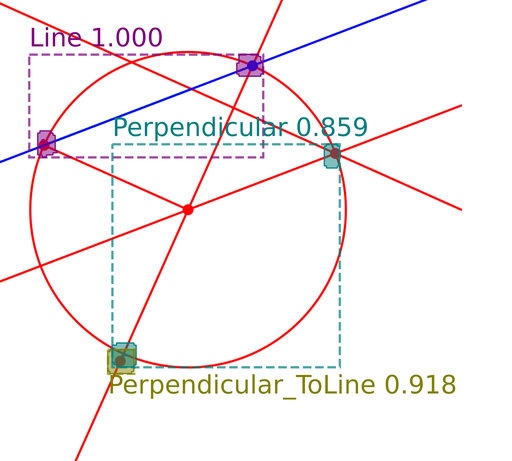
\includegraphics[width=\textwidth]{img/Gamma-08_example/output_image4.png}
         \caption{Step 5: Line tool}
         \label{fig:Gamma08_example_step5}
     \end{subfigure}
     \hfill
     \begin{subfigure}[t]{0.32\textwidth}
         \centering
         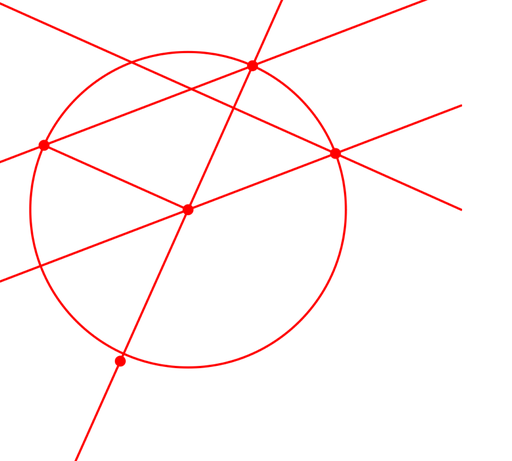
\includegraphics[width=\textwidth]{img/Gamma-08_example/input_image5.png}
         \caption{Construction finished}
         \label{fig:Gamma08_example_step6}
     \end{subfigure}
     
        \caption{Example construction of Euclidea level \textit{Gamma-08} (construct a rhombus with the given side and an angle of $45^\circ$ in a vertex). The figure contains 5 steps of the construction. (a) Definition of the problem. (b-f) Construction steps containing \maskrcnn detections of possible steps. In each subfigure, the red color denotes the current state of the construction, green the remaining goals, blue the geometric primitive proposed by the detection,
        and other
        colors mark the prediction masks, bounding boxes, classes and scores for the predicted action.
        }
        \label{fig:Gamma08_example}
\end{figure}
\newpage
\subsection{Level \textit{Delta-10}}
\begin{figure}[!htb]
     \centering
     \begin{subfigure}[t]{0.32\textwidth}
         \centering
         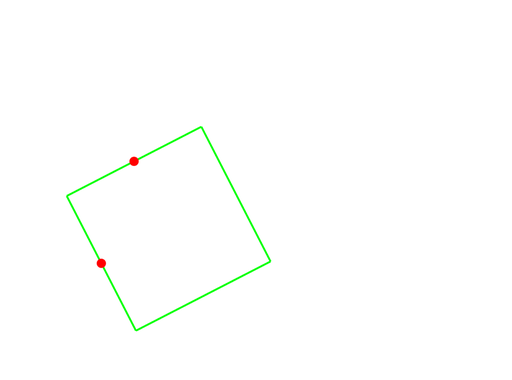
\includegraphics[width=\textwidth]{img/Delta-10_example/input_image0.png}
         \caption{Input}
         \label{fig:Epsilo12_example_input}
     \end{subfigure}
     \hfill
     \begin{subfigure}[t]{0.32\textwidth}
         \centering
         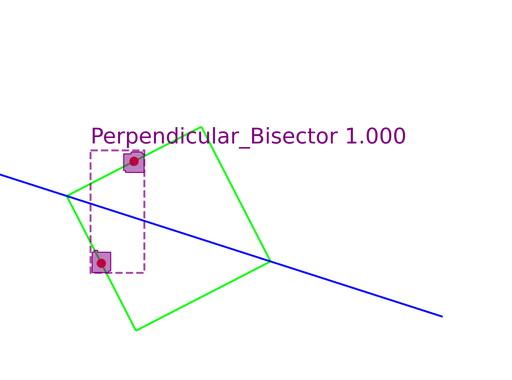
\includegraphics[width=\textwidth]{img/Delta-10_example/output_image0.png}
         \caption{Step 1: Perpendicular Bisector tool}
         \label{fig:Epsilon12_example_step1}
     \end{subfigure}
     \hfill
     \begin{subfigure}[t]{0.32\textwidth}
         \centering
         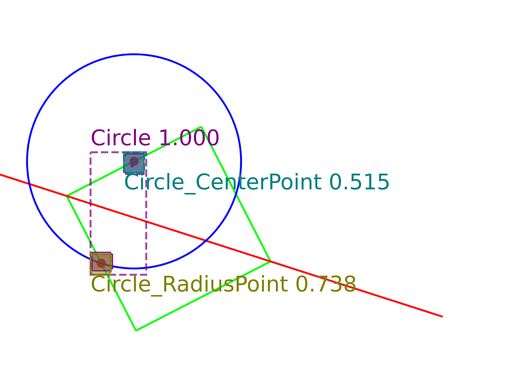
\includegraphics[width=\textwidth]{img/Delta-10_example/output_image1.png}
         \caption{Step 2: Circle tool}
         \label{fig:Epsilon12_example_step2}
     \end{subfigure}
     \hfill
     \begin{subfigure}[t]{0.32\textwidth}
         \centering
         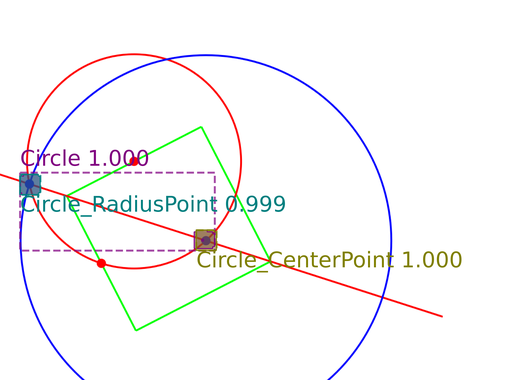
\includegraphics[width=\textwidth]{img/Delta-10_example/output_image2.png}
         \caption{Step 3: Circle tool}
         \label{fig:Epsilon12_example_step3}
     \end{subfigure}
     \hfill
     \begin{subfigure}[t]{0.32\textwidth}
         \centering
         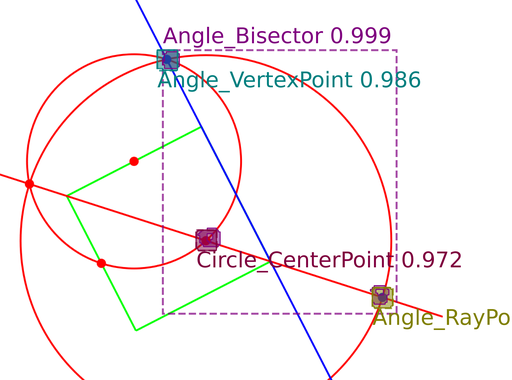
\includegraphics[width=\textwidth]{img/Delta-10_example/output_image3.png}
         \caption{Step 4: Angle Bisector tool}
         \label{fig:Epsilon12_example_step4}
     \end{subfigure}
     \hfill
     \begin{subfigure}[t]{0.32\textwidth}
         \centering
         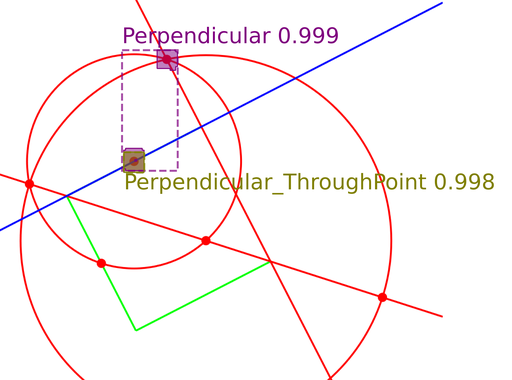
\includegraphics[width=\textwidth]{img/Delta-10_example/output_image4.png}
         \caption{Step 5: Perpendicular tool}
         \label{fig:Epsilon12_example_step5}
     \end{subfigure}
     
     \begin{subfigure}[t]{0.32\textwidth}
         \centering
         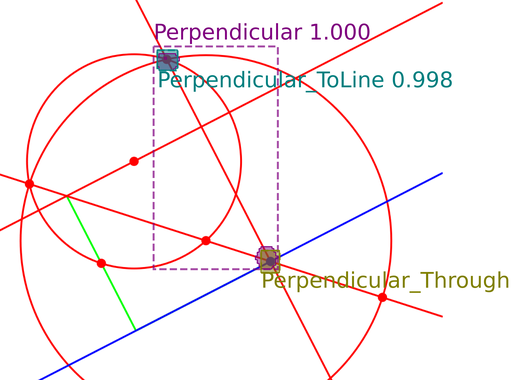
\includegraphics[width=\textwidth]{img/Delta-10_example/output_image5.png}
         \caption{Step 6: Perpendicular tool}
         \label{fig:Epsilon12_example_step6}
     \end{subfigure}
     \hfill
     \begin{subfigure}[t]{0.32\textwidth}
         \centering
         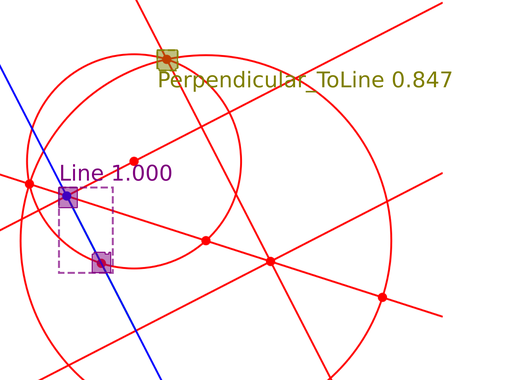
\includegraphics[width=\textwidth]{img/Delta-10_example/output_image6.png}
         \caption{Step 7: Line tool}
         \label{fig:Epsilon12_example_fin}
     \end{subfigure}
     \hfill
     \begin{subfigure}[t]{0.32\textwidth}
         \centering
         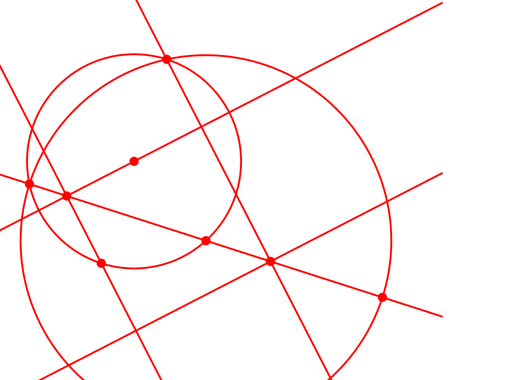
\includegraphics[width=\textwidth]{img/Delta-10_example/input_image7.png}
         \caption{Construction finished}
         \label{fig:Epsilon12_example_fin}
     \end{subfigure}
     \hfill
     
        \caption{Example construction of Euclidea level \textit{Delta-10} (construct a square by adjacent side midpoints). The figure contains 7 steps of the construction. (a) Definition of the problem. (b-h) Construction steps containing \maskrcnn detections of possible steps. In each subfigure, the red color denotes the current state of the construction, green the remaining goals,
        blue the geometric primitive proposed by the detection,
        and other
        colors mark the prediction masks, bounding boxes, classes and scores for the predicted action hypotheses.
        }
        \label{fig:Delta10_example}
\end{figure}
\newpage
\subsection{Level \textit{Zeta-12}}
\begin{figure}[htb!]
     \centering
     \begin{subfigure}[t]{0.32\textwidth}
         \centering
         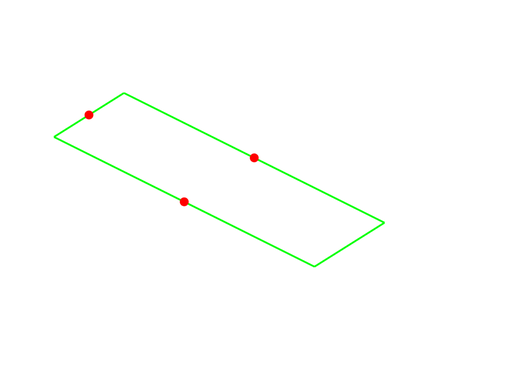
\includegraphics[width=\textwidth]{img/Zeta-06_example/input_image0.png}
         \caption{\small Input.}
         \label{fig:Zeta06_example_input}
     \end{subfigure}
     \hfill
     \begin{subfigure}[t]{0.32\textwidth}
         \centering
         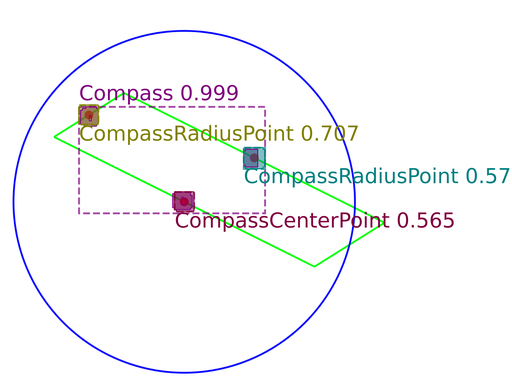
\includegraphics[width=\textwidth]{img/Zeta-06_example/output_image0.png}
         \caption{\small Step 1: Compass tool.  
         The Compass tool requires two radius points and one center point.)
         }
         \label{fig:Zeta06_example_step1}
     \end{subfigure}
     \hfill
     \begin{subfigure}[t]{0.32\textwidth}
         \centering
         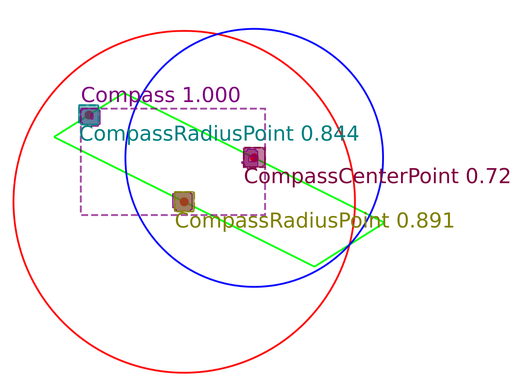
\includegraphics[width=\textwidth]{img/Zeta-06_example/output_image1.png}
         \caption{\small Step 2: Compass tool. 
         (Note that the center point is detected elsewhere than in the last step.)
         }
         \label{fig:Zeta06_example_step2}
     \end{subfigure}
     \hfill
     \begin{subfigure}[t]{0.32\textwidth}
         \centering
         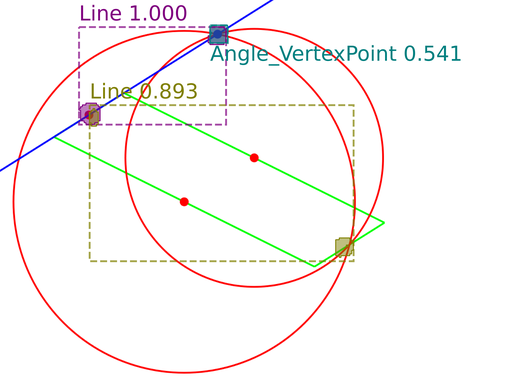
\includegraphics[width=\textwidth]{img/Zeta-06_example/output_image2.png}
         \caption{\small Step 3: Line tool.}
         \label{fig:Zeta06_example_step3}
     \end{subfigure}
     \hfill
     \begin{subfigure}[t]{0.32\textwidth}
         \centering
         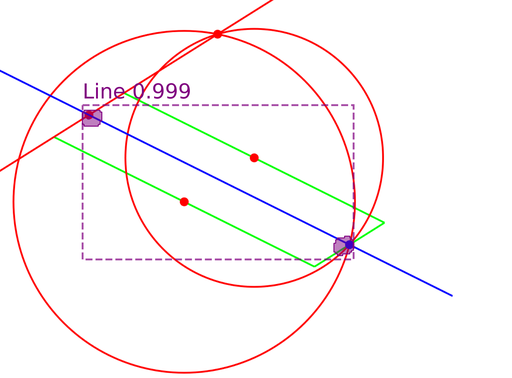
\includegraphics[width=\textwidth]{img/Zeta-06_example/output_image3.png}
         \caption{\small Step 4: Line tool. }
         \label{fig:Zeta06_example_step4}
     \end{subfigure}
     \hfill
     \begin{subfigure}[t]{0.32\textwidth}
         \centering
         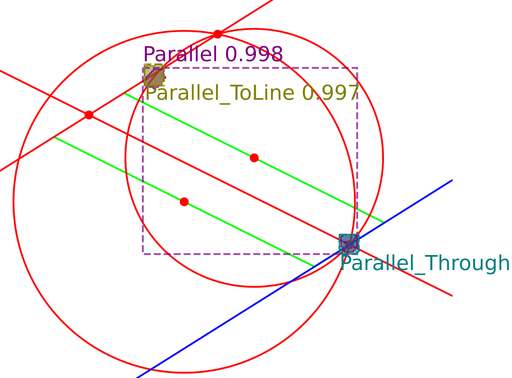
\includegraphics[width=\textwidth]{img/Zeta-06_example/output_image4.png}
         \caption{\small Step 5: Parallel tool.}
         \label{fig:Zeta06_example_step5}
     \end{subfigure}
     \hfill
     \begin{subfigure}[t]{0.32\textwidth}
         \centering
         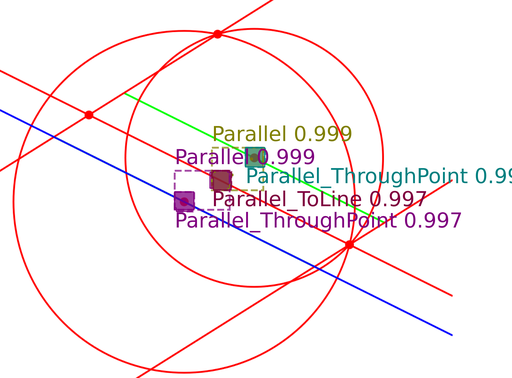
\includegraphics[width=\textwidth]{img/Zeta-06_example/output_image5.png}
         \caption{\small Step 6: Parallel tool.}
         \label{fig:Zeta06_example_step6}
     \end{subfigure}
     \hfill
     \begin{subfigure}[t]{0.32\textwidth}
         \centering
         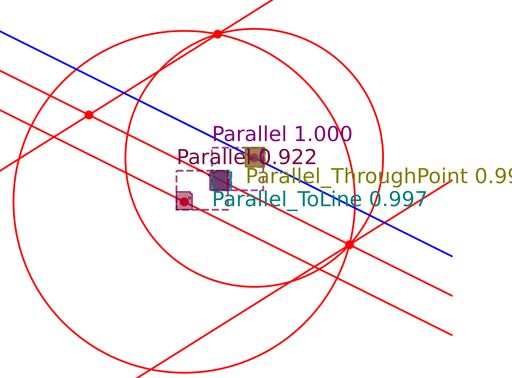
\includegraphics[width=\textwidth]{img/Zeta-06_example/output_image6.png}
         \caption{\small Step 7: Parallel tool.}
         \label{fig:Zeta06_example_step7}
     \end{subfigure}
     \hfill
     \begin{subfigure}[t]{0.32\textwidth}
         \centering
         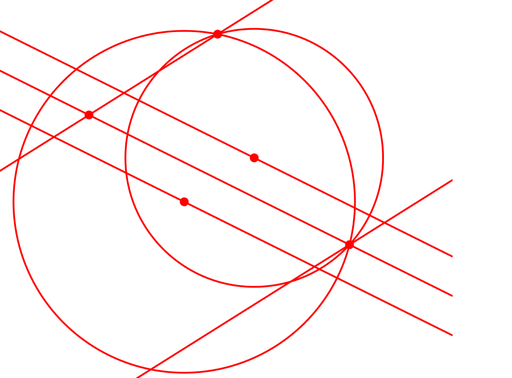
\includegraphics[width=\textwidth]{img/Zeta-06_example/input_image7.png}
         \caption{\small Construction finished.}
         \label{fig:Zeta06_example_finished}
     \end{subfigure}
     \hfill
        \caption{\small Example construction of Euclidea level \textit{Zeta-12} (construct a parallelogram given three of the midpoints).
        The figure contains 7 steps of the construction. (a) Definition of the problem. (b-h) Construction steps containing \maskrcnn detections of possible steps. In each subfigure, the red color denotes the current state of the construction, green the remaining goals, blue the geometric primitive proposed by the detection,
        and other
        colors mark the prediction masks, bounding boxes, classes and scores for the predicted action hypotheses.
        }
        \label{fig:Zeta06_example}
\end{figure}
